\documentclass[12pt]{standalone}

\usepackage{tikz}
\usepackage{ctex}

\begin{document}
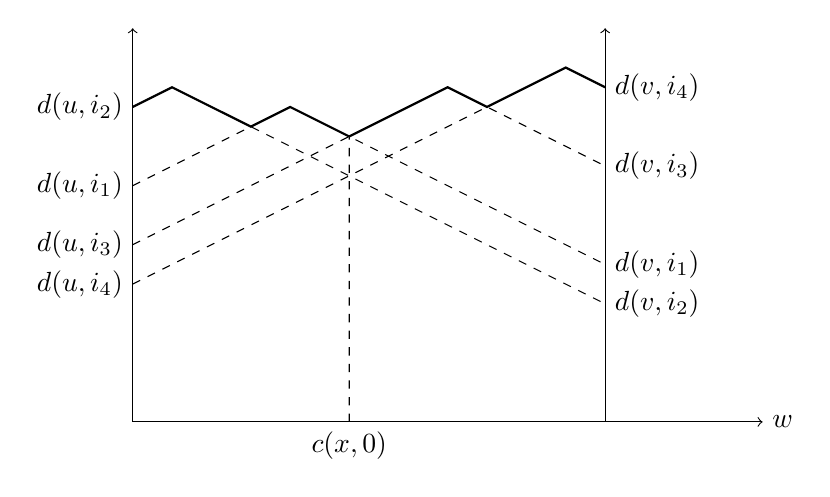
\begin{tikzpicture}

% the coordinates frame

\draw[->] (0,0) -- (0,5);
\draw[->] (6,0) -- (6,5);
\draw[->] (0,0) -- (8,0) node[right] {$w$};

% the plot

\draw[dashed] (0,3) node[left] {$d(u,i_1)$}
    -- (2,4) -- (6,2) node[right] {$d(v,i_1)$};
\draw[dashed] (0,4) node[left] {$d(u,i_2)$}
    -- (0.5,4.25) -- (6,1.5) node[right] {$d(v,i_2)$};
\draw[dashed] (0,2.25) node[left] {$d(u,i_3)$}
    -- (4,4.25) -- (6,3.25) node[right] {$d(v,i_3)$};
\draw[dashed] (0,1.75) node[left] {$d(u,i_4)$}
    -- (5.5,4.5) -- (6,4.25) node[right] {$d(v,i_4)$};

\coordinate (I12) at (intersection cs:
    first line={(0,3)--(2,4)},second line={(0.5,4.25)--(6,1.5)});
\coordinate (I13) at (intersection cs:
    first line={(0,2.25)--(4,4.25)},second line={(2,4)--(6,2)});
\coordinate (I34) at (intersection cs:
    first line={(4,4.25)--(6,3.25)},second line={(0,1.75)--(5.5,4.5)});

\draw[thick] (0,4) -- (0.5,4.25) -- (I12) -- (2,4)
    -- (I13) -- (4,4.25) -- (I34) -- (5.5,4.5) -- (6,4.25);

\draw[dashed] (2.75,0) node[below] {$c(x,0)$} -- (I13);

\end{tikzpicture}
\end{document}
